\subsection{Normals > Compute}
\label{subsection:computeNormals}

\begin{figure}[!htb]
\begin{center}
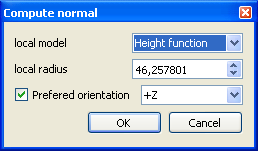
\includegraphics[width=0.4\textwidth]{Partie3_Fonctions/computeNormalsDlg.png}
\caption{\label{fig:computeNormalsDlg}Interface pour le calcul des normales}
\end{center}
\end{figure}

\index{normales}
\textcolor{red}{Cette fonction ne permet pas de calculer des normales sign�es. Pour ceci utilisez la m�thode \textit{Estimate Normals and Curvature} de la librairie PCL via le plugin qPCL (voir \ref{subsection:qPCL}).}
\\
\par
Cette fonction permet de calculer les normales (non sign�es) d'un nuage de points.\\
\par
L'utilisateur peut sp�cifier le mod�le d'approximation locale de la surface parmi :
\begin{itemize}
\item Plane : plan aux moindres carr�s (le plus rapide)
\item Height function : quadrique (le plus pr�cis)
\item Triangulation : triangulation 2D$\frac{1}{2}$ de type Delaunay (int�rm�diaire)\\
\end{itemize}

L'utilisateur doit aussi sp�cifier la taille du voisinage pour la mod�lisation locale (\textit{local radius} : plus celui-ci est grand et plus le r�sultat sera lisse ... et le calcul lent).\\

Enfin, si une direction privil�gi�e pour les normales est disponible, l'utilisateur peut la sp�cifier pour aider CloudCompare � \textit{signer} les normales. Il faut activer la case � cocher \textsl{Prefered orientation} et sp�cifier une des 6 orientations par d�faut (-X,+X,-Y,+Y,-Z,+Z). Autrement, l'utilisateur peut tenter sa chance aupr�s de la m�thode \emph{Resolve direction} (Cf. section~\ref{subsection:resolveNormalsDirection}).
